%%%%%%%%%%%%%%%%%%%%%%%%%%%%%%%%%%%%%%%%%%%%%%%%%%%%%%%%%%%%%%%%%%%%%%%%%%%%%%%%
%2345678901234567890123456789012345678901234567890123456789012345678901234567890
%        1         2         3         4         5         6         7         8

\documentclass[letterpaper, 10 pt, conference]{ieeeconf}  % Comment this line out
                                                          % if you need a4paper
%\documentclass[a4paper, 10pt, conference]{ieeeconf}      % Use this line for a4
                                                          % paper

\IEEEoverridecommandlockouts                              % This command is only
                                                          % needed if you want to
                                                          % use theplp \thanks command
\overrideIEEEmargins
% See the \addtolength command later in the file to balance the column lengths
% on the last page of the document



% The following packages can be found on http:\\www.ctan.org
\usepackage{graphics} % for pdf, bitmapped graphics files
\usepackage{epsfig} % for postscript graphics files
\usepackage{mathptmx} % assumes new font selection scheme installed
\usepackage{times} % assumes new font selection scheme installed
\usepackage{amsmath} % assumes amsmath package installed
\usepackage{amssymb}  % assumes amsmath package installed
\usepackage[noadjust]{cite}
\usepackage{dblfloatfix}
\usepackage{color}
\renewcommand{\thefigure}{\arabic{figure}}

\title{\LARGE \bf
Design of a Soft Elbow Exosuit for Lifting Assistance
}

%\author{ \parbox{3 in}{\centering Huibert Kwakernaak*
%         \thanks{*Use the $\backslash$thanks command to put information here}\\
%         Faculty of Electrical Engineering, Mathematics and Computer Science\\
%         University of Twente\\
%         7500 AE Enschede, The Netherlands\\
%         {\tt\small h.kwakernaak@autsubmit.com}}
%         \hspace*{ 0.5 in}
%         \parbox{3 in}{ \centering Pradeep Misra**
%         \thanks{**The footnote marks may be inserted manually}\\
%        Department of Electrical Engineering \\
%         Wright State University\\
%         Dayton, OH 45435, USA\\
%         {\tt\small pmisra@cs.wright.edu}}
%}

\author{Carly M. Thalman$^{1*}$, \textit{Student Member, IEEE}, Quoc P. Lam$^{1*}$, Pham H. Nguyen$^{1}$, \textit{Student Member, IEEE}, 
\\Saivimal Sridar$^{1}$, \textit{Student Member, IEEE}, and Panagiotis Polygerinos$^{1**}, \textit{Member, IEEE}$% <-this % stops a space
\thanks{*Equally Contributing 1st Authors}% <-this % stops a space
\thanks{**Corresponding Author}% <-this % stops a space
\thanks{$^{1}$ Carly M. Thalman, Quoc P. Lam, Pham H. Nguyen, Saivimal Sridar, and Panagiotis Polygerinos are with the Polytechnic School, Ira A. Fulton Schools of Engineering, Arizona State University, Mesa, AZ 85212, USA.
        {\tt\small cmthalma@asu.edu, qlam1@asu.edu, nhpham2@asu.edu, ssridar@asu.edu, polygerinos@asu.edu}}%
}



\begin{document}



\maketitle
\thispagestyle{empty}
\pagestyle{empty}


%%%%%%%%%%%%%%%%%%%%%%%%%%%%%%%%%%%%%%%%%%%%%%%%%%%%%%%%%%%%%%%%%%%%%%%%%%%%%%%%
\begin{abstract}

This paper investigates the design of a soft robotic elbow exosuit capable of providing supplemental lifting assistance to the elbow joint.  The aim is to improve the efficiency and endurance of workers who are tasked with repetitive lifting. The design consists of an array of pneumatically pressurized actuators, which are encased in a nylon fabric casing to allow for high force-to-weight ratios. An analytical model governing the torque production of the device is created, where testing results were within 10\% agreement with the theoretical model. A torque value of 27.6 $N \cdot m$ is achieved at 275kPa. Further testing with a healthy participant was also conducted using electromyography sensors and a motion capture system to assess the performance of the exosuit. Measurable assistance to lifting with minimal impedance to the user is observed in all tests. With an experimentally validated model and a range of potential applications for this assistive soft elbow exosuit, our hopes are to further develop this technology and in the future, implement it in a multitude of ways.    



\end{abstract}


%%%%%%%%%%%%%%%%%%%%%%%%%%%%%%%%%%%%%%%%%%%%%%%%%%%%%%%%%%%%%%%%%%%%%%%%%%%%%%%%
\section{INTRODUCTION}

Freight, stock, and warehouse workers are required to perform strenuous and repetitive tasks like packing, shelving, loading, and unloading goods on a daily basis. These repetitive motions can lead to fatiguing, as well as lower-back and upper-limb injuries that reduces productivity. Injuries in this line of work are generally musculoskeletal disorders (MSDs) that can be caused by improper lifting postures, repetitive high strain activities, and age-related factors \cite{BLS2017}.

According to the US Department of Labor in 2015, there were 376,190 cases (33\% of all injury cases) of MSDs caused by overexertion in lifting \cite{BLS2016}. Of all the occupations, laborers and freight, stock, and material movers were part of the highest number of injury cases in 2015 \cite{BLS2016}. The cost of workplace injury in the USA amounted to be around \$190 billion and has resulted in over 1.1 million lost days of work \cite{Leigh2011}. There has also been a consistent increase in the age of the labor force since the beginning of the century (the median age is around 48 years old) and the 45 and over category of workers have grown from 34\% to 44\% of the total labor force, since 2000 \cite{Mislinski2017}. 

\begin{figure}[t!]
\centering
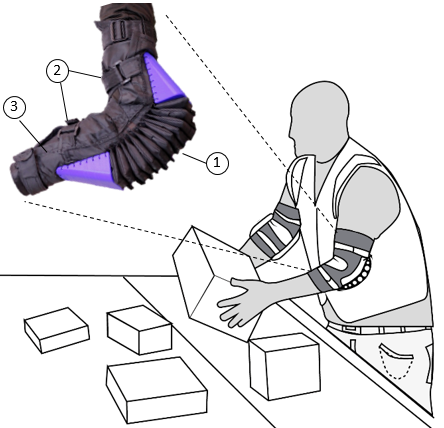
\includegraphics[width=0.5\textwidth]{Concept.PNG}
\caption{Illustrated concept of the soft robotic elbow exosuit warehouse environment. Key design elements include: (1) Straps to tighten and loosen the exosuit. (2) Network of actuators for flexion motion of elbow.  (3) Elastic elbow-sleeve to attach exosuit to user’s arm.}
\label{fig:concept}
\vspace{-1.5em}
\end{figure}

Potential solutions for approaching this problem have been seen in the field of wearable robotics and human augmentation. Human augmentation robotic devices are designed to help augment load carriage capacity and normal muscle function in healthy individuals while reducing the amount of physical exertion the user is required to sustain. Examples of human augmentation via exoskeletons have been seen for multi-purposes in healthcare, rehabilitation, and industrial settings \cite{Kazerooni2008}. There have been a variety of lower-limb exoskeletons \cite{Viteckova2013} and upper-limb devices \cite{Gopura2016a}. These devices seek to increase the load bearing capability of the user. The primary concerns of using exoskeletons is with their rigidity, high cost, portability, alignment complications with the biological joint it is trying to assist, and the comfort over long periods of use.

The recent introduction and advancement of soft robotics has led to promising designs of wearable devices that are compliant, safe for human-robot interaction, lightweight, low-cost to fabricate, allows even distribution of force on the users joints, and are unaffected by alignment issues like with rigid exoskeletons \cite{ADEM:ADEM201700016}. These intrinsically soft wearable devices have been categorized based on their novel form of actuation, including cable-driven actuators \cite{Gopura2016a} \cite{Dinh2017} \cite{Xiloyannis2017} \cite{Ding2016}, pneumatic artificial muscles \cite{Park2014cd},\cite{CALDWELL2007a} \cite{Al-fahaam2017}, fluidic elastomeric actuators\cite{Polygerinos,Koh2017,Chen2017h}, and pneumatically inflatable bladder-based actuators \cite{Kim2017,Sridar2017,Simpson2017,Koh2017}.

The design of the proposed soft elbow exosuit is aimed at providing assistance during activities involving elbow flexion, such as lifting and manipulating heavy objects within an industrial setting. Ergonomics are taken into consideration where the goal is to create a low-profile design that does not limit the user’s range of motion (ROM). 

The average male, aged 24.4 $\pm$ 2.2 years, is capable of producing an average of 60 $N \cdot m$ of torque, at a 90$^o$ bend. \cite{sardelli2011functional}. For the average female, however, this torque values is 34 $N \cdot m$ at maximum, or nearly half that of the average male \cite{laksanacharoen2003design}. Rather than design the exosuit to accommodate to specific genders, the exosuit was designed to assist for torque values based on the safe maximum threshold of 30 $N\cdot{m}$, set by OSHA requirements in the US, which is roughly 11kg per arm \cite{waters1994applications} .  

\section{DESIGN OF THE SOFT ELBOW EXOSUIT}

A network of small cylindrical actuators are arranged in an array and fixed with an inextensible fabric layer between the base of each actuator as shown in Fig. \ref{fig:array} (c) and (d).  When the array inflates, the interaction of the expanding actuators produces a bending motion as the rotation is constrained along the base (Fig. \ref{fig:array} (a) and (b)).  This methodology has been successfully proven to achieve predictable bending patterns using  individual actuators created by hermetically sealing the borders of two sheets of thermoplastic polyurethane (TPU) material \cite{mosadegh2014pneumatic}\cite{ADEM:ADEM201700016}\cite{natividad2017h} \cite{Koh2017}.    However, by encasing these type of actuators in an inextensible, weaved nylon material of the same net shape, the actuators can sustain higher pressures as they are no longer limited by the low tensile strength of the TPU during inflation .  This allows for a novel approach to obtaining higher force-to-weight ratios from a single actuator than previously possible using TPU-based inflatable actuators.  
% Please add L and w to figure 1a.
\begin{figure}[t]
\centering
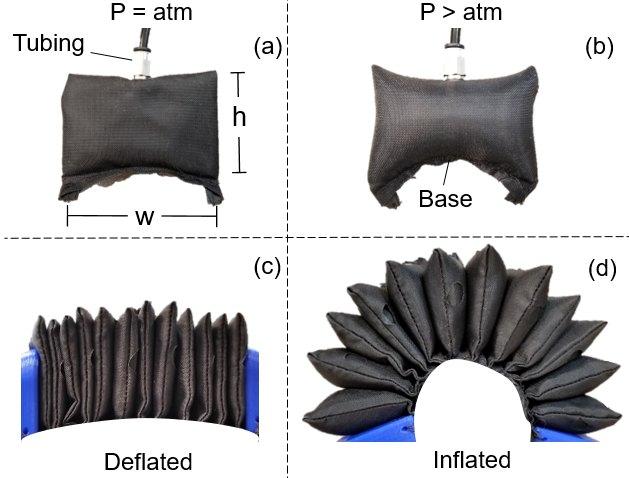
\includegraphics[width=0.5\textwidth]{V1_device.PNG}
\caption{(a) Deflated Actuator. (b) Inflated Actuator. (c) Deflated actuator array, constrained with end stops at each side. (d) Inflated actuator array conforming around inextensible fabric along the inner radius of bending, constrained with end stops on either side.
}
\vspace{-1.5em}
\label{fig:array}
\end{figure}

\begin{figure}
\centering
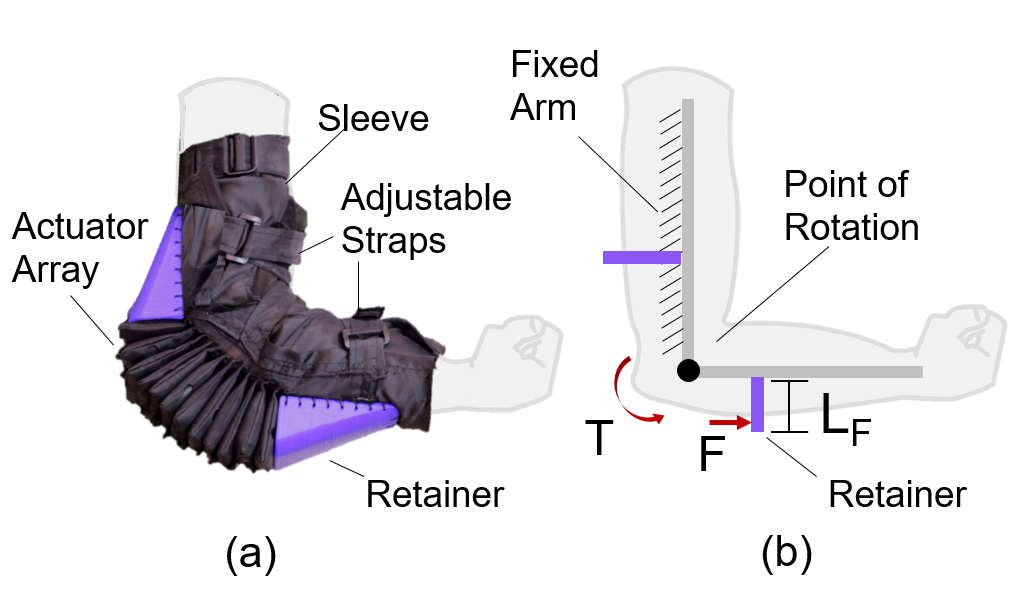
\includegraphics[width=0.4\textwidth]{arm.PNG}
\caption{Final Design of the soft robotic elbow sleeve (left) worn by a user, and the basic torque model concept behind the device (right)}
\label{fig:arm}
\vspace{-1.5em}
\end{figure}
 
 
 

 
 
 The design of the exosuit aims maintain to full ROM in which tasks of daily living and working are performed \cite{sardelli2011functional}.   To keep the exosuit design lightweight, an upper limit of 2.3 kg is set - the average weight of the male forearm and hand combined \cite{clauser1969weight}.    Consideration is given to the manufacturing process, where sewing actuators in close proximity can prove to be difficult. Therefore the distance between each actuator is limited of a minimum of 5mm. Possible angles between two actuators have been limited to $90^{\circ}$ as the bending angle becomes asymptotic at this point, where the distance starts to become negligible and . It was assumed that an actuator with a height of more than 50mm would exceed that of a low-profile exosuit.  
 

 
 % In the conclusion, discuss the total device mass. Otherwise we just say "lightweight" as Sai suggested, because "2.3 kg is still heavy".
 

 \subsection{Fabrication}
 At its general form, the proposed actuator design uses an array of hermetically sealed, and nylon encased actuators proximally mounted to the backside of the elbow joint.   The TPU  (DT-2001, American Polyfilm, Branford, CT) is sealed with a modified soldering iron at $550^{\circ}$F for the complex curvature of the base seal, and finished with an impulse sealer (model make location) once internal fittings had been attached.  A laser cutter (Glowforge Pro, Glowforge, Seattle, WA) is used to cut the nylon material into the desired shape, where it is sewn into its final shape with the use of an embroidery sewing machine (model Brother, Bridgewater, NJ).  The sewing machine tends to show a tolerance of $\pm1mm$ during fabrication and factored into the final theoretical model for torque output. 
 % First sentence redundant. kind of. same thing is said in the first paragraph of design. 

\section{Theoretical Modeling}

\subsection{Modeling Bending Angle}

\begin{figure}[t!]
\centering
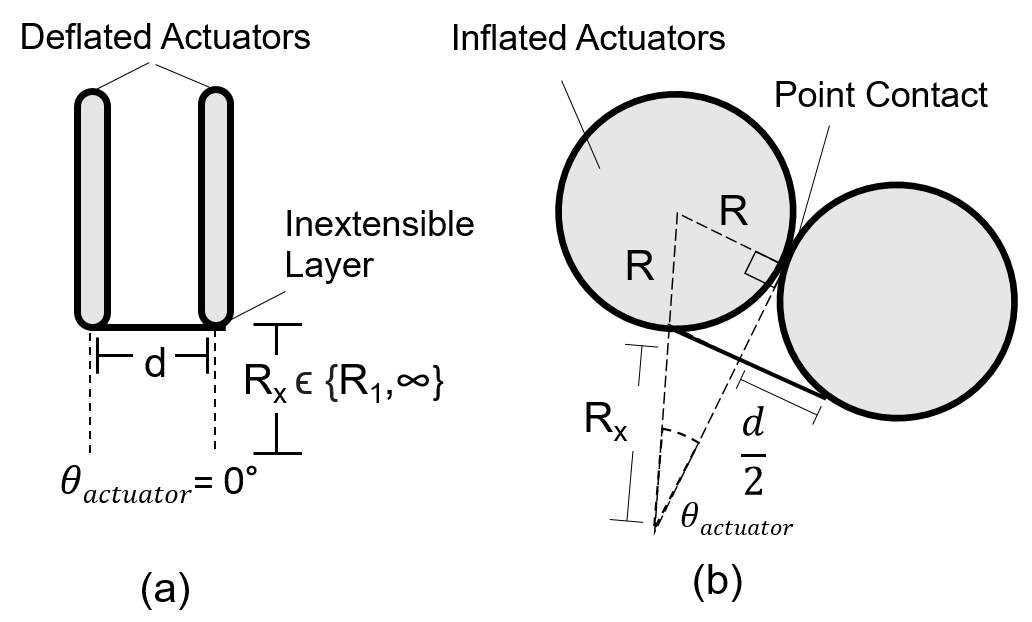
\includegraphics[width=0.4\textwidth]{ActuatorModel1.PNG}
\caption{(a) Model of two adjacent actuators in a deflated state, where no contact occurs.  (b) Two-dimensional geometric model of two adjacent actuators when fully pressurized}
\label{fig:Model1}

\end{figure}

The array of actuators is symmetrical and simplified to a two-dimensional model shown in Fig. \ref{fig:Model1}. When in a fully deflated state, the actuators are assumed to have no contact with adjacent actuators in the array as shown in Fig. \ref{fig:Model1}(a). The interaction between two actuators is modeled using the following assumptions: the individual actuators inflate to create a circular cross section, the deformation when fully pressurized is negligible, a point contact will form with adjacent actuators, and the actuators are fixed at a point to the inextensible layer [Fig. \ref{fig:Model1}(b)].  The following model is used to select the appropriate range of parameters for radius of individual actuators, $R$, and the spacing between consequent individual actuators, $d$.  A constraint was set limiting $d$ to be less than the diameter of each inflated actuator in order to ensure the point contact would occur to induce a bending angle, $\theta$, where $ 2R > d$. 

\begin{equation}\label{eq. sin}
	\theta=sin^{-1}(1-d/2R) 
\end{equation}

Using Eq. \ref{eq. sin} the set boundary conditions, and adding taking manufacturing constraints into consideration, the range for $d$ and $R$ were determined with a combination of the two graphs shown in Fig. \ref{fig:Graphs1}.   
 
Figure\ref{fig:Graphs1} shows $\theta$ with various fixed $R$ and distance values, where observation of the behavior of the model allowed for selection of the parameters used in following force and torque models, as a starting guideline.  Increasing $R$ is observed for various fixed $d$ in Fig. \ref{fig:Graphs1}(a), showing higher $R$ values correlate to increasing  $\theta$ values.  Figure \ref{fig:Graphs1}(b) shows increasing $d$ at various fixed $R$ values.  It is observed that $d$ and $\theta$ have an inverse relationship.  The specific boundary conditions for manufacturing the exosuit are shaded, leaving the feasible dimensions left unshaded.  The ratio of $R$ /$d$  is what governs $\theta$, therefore for the following torque model, only the higher values of $R$ are considered, ranging from 12.5mm to 16mm based on the circumference of a flattened actuator to achieve height (40mm and the maximum height of 50mm respectively).  Based on these values, $d$ will be minimized.


\begin{figure}
\centering
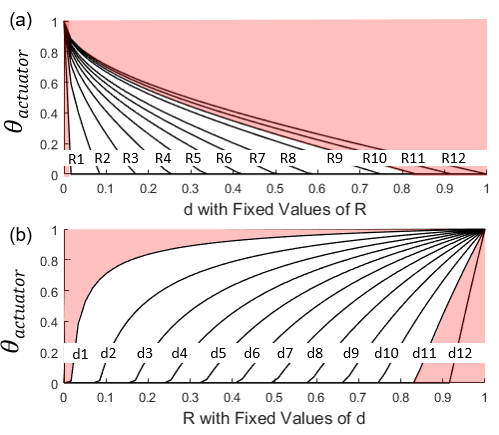
\includegraphics[width=0.5\textwidth]{graphs_model1.PNG}
\caption{This model assumes that each actuator has reached a steady-state pressure and will not deform during bending.  It is also assumed that each actuator will inflate to form a perfect circle.  (a) shows the relationship between bending angle and a changing actuator radius given a fixed distance between each bladder.  (b) shows the relationship between bending angle and a changing distance given a fixed radius.}
\label{fig:Graphs1}

\end{figure}	

\subsection{Modeling Torque Output of Actuator Array}

%\begin{equation}\label{eq. X16}
%	F = PLw 
%\end{equation}

% need to talk about pressure force length and width in the design section. keep high high level, only enough for the reader to understand the thought process behind torque generation

\begin{figure}[t!]
\centering
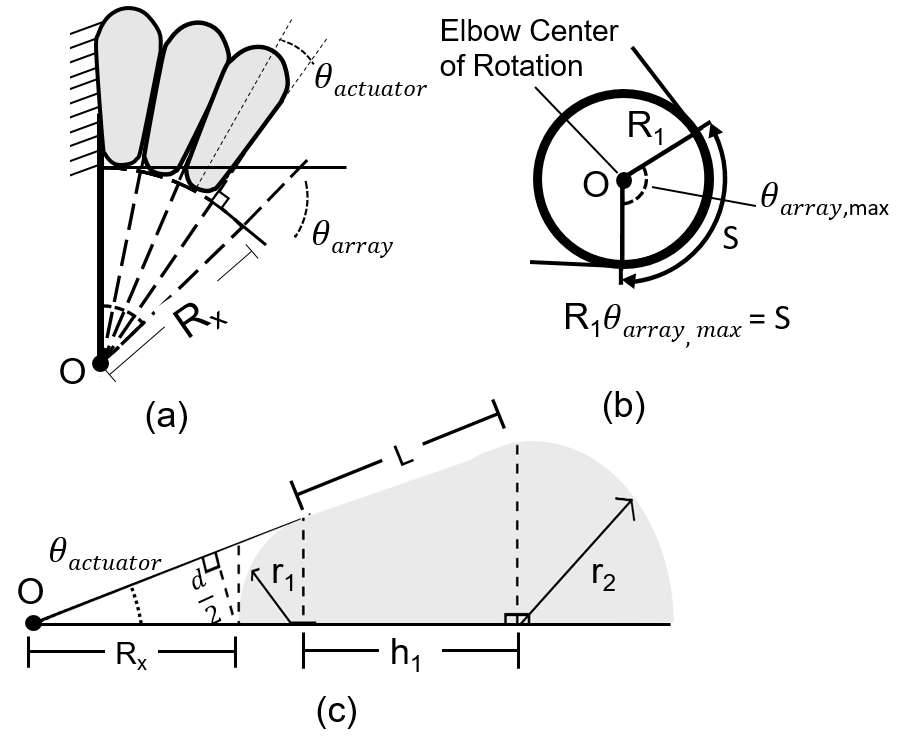
\includegraphics[width=0.4\textwidth]{model3.PNG}
\caption{(a) Arc length model used to determine total actuator length. (b) Simple two bladder arrangement demonstrating $R_x = \infty$. (c) The inextensible layer joining adjacent bladders at the base of the device, with length, $d$, is assumed to be curved as it cumulatively arches to reach the elbow bending angle, $\theta_0$ }
\label{fig:hotness}
\end{figure}

Modeling torque about the actuators follow the same geometric principles outlined in Section IVa. However, line contact across two actuators is replaced with the interacting area to account for shape deformation. Assuming the exosuit is pressurized with ideal expansion of the actuators, the resultant shape of individual actuators become constrained and identical to one other (Fig \textcolor{red}{BOOM (A)}). This assumption is made on the premise of the elbow joint modeled as a sphere of radius, $R_1$.  The total length is the arc length, $S$, the array is proportional to $R_1$ and the maximum bending angle of the elbow, $\theta_{max}$.
% remember to have the pleated image on the left for (a)

\begin{equation}\label{S}
	S = R_1\theta_{max}.
\end{equation}

\begin{equation}\label{Rx1}
	R_x(\theta_0) = \frac{S}{\theta_0}
\end{equation}

\begin{equation}\label{Rx2}
	R_x(\theta_0) = R_1\frac{\theta_{max}}{\theta_0}
\end{equation}

\begin{figure}[b!]
\centering
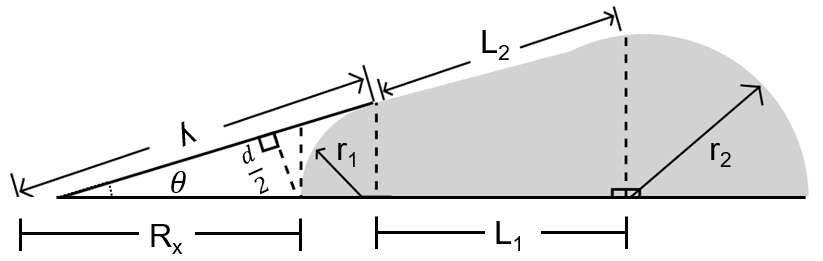
\includegraphics[width=0.4\textwidth]{Models_Torque.PNG}
\caption{Two-dimensional representation of the half-section of an actuator inflated against the adjacent ones. All variables listed were used in calculating the reactionary forces produced. }
\label{fig:nomenclature}
\end{figure}

Unlike the constant elbow joint radius, it is necessary to define a radius of curvature for the total array, $R_x$. The angle of $S$ is equal to the elbow joint angle, $\theta_0$, and therefore substitution of Eq \ref{S} into Eq \ref{Rx1} results in $R_x$ being dependent on $R_1$ and $\theta_0$.  Figure \textcolor{red}{BOOM B} demonstrates that the range of $R_x$ must vary from ${\infty}$ to $R_{1}$ as the elbow bends from full extension through its full range of motion as it has an inverse dependence on $\theta_0$.    

Since the actuators are symmetrical about the radial centerline, the cross-section, shown in \textcolor{red}{BOOM A}, is used to extract dimensions needed to calculate their reaction forces (Fig. .  The minor angle, $\theta_1$, is introduced to represent the angle between the centerline of an actuator and its edge in contact with the adjacent actuator. It is equivalent to $\theta_0/2n$, where $n$ is the quantity of equidistant actuators along $S$.  The spacing between actuators, $d$, is driven by the quantity $n$, and length of $S$ by the relationship $n/S$. 

\begin{equation}\label{r1}
	r_1(\theta_1)  = \frac{dR_x}{2R_xcos(\frac{\theta_1}{2\textit{n}})}
\end{equation}\label{r2}
 \begin{equation}
	r_2(\theta_1)  = -b + \sqrt{\frac{b^2-4ac}{2a}}
\end{equation}
\begin{equation}\label{L}
	 \pi R = \frac{\pi}{2}(r_1+r_2) + L(\theta_1),
\end{equation}



The inner radius, $r_1$, is found through its tangent relationship with respect to $d$, and $R_x$; $r_2$ is found utilizing the same trigonometric function in addition to simple geometrical substitutions that lead to $r_2$ reducing to a second order polynomial. The quadratic solution is shown in Eg. \textcolor{red}{BOOM}. The length of interaction, $L$, and perimeter of quarter-circle, $r_1$ and $r_2$ is related to the perimeter of a semi-circle, or $\pi R$, by Eq \textcolor{red}{BOOM }. 
%Equations \textcolor{red}{BOOM} and \textcolor{red}{BOOM} is input into Eq. \textcolor{red}{BOOM BOOM} to find the $L$. 




An adjusted effective width, $w_1$, is required to better represent the behavior of the actuators as the exosuit 


The rectangular actuators do not form a perfect cylinder due to the boundary conditions of the structure, witnessed in previous work with inflatable actuators (\cite{Natividad2017}). Therefore, an approximation is made on the effective width, $w_1$, in contact. It was assumed that reduction from initial width, $w_0$, is dependent on the ratio of the inflated actuator's height, $h_1$ to initial height, $h_0$ (eq. 8).

\begin{equation}\label{w1}
	w_1(\theta_1)  = w_0-2R(1-\frac{h_1(\theta_1)-2R}{h_0-2R})
\end{equation}

Once $\textit{L}$ was determined, the effective force was calculated, and therefore, the torque it would generate about the elbow joint. Since pressure, $\textit{P}$ is equal at every point within the inside of the actuator, force, $\textit{F}$ is also distributed evenly across the interacting area ($L\cdot w_{1}$) and is represented as a point load applied at $L_f$, the distance from the axis of rotation to the center of $L$.

Various inputs, i.e. actuator heights, quantity of actuators and a 90 degree bending angle, were used to assess their resultant torque values (Fig. 8). The three main considerations for inputs were based on design constraints in which the remaining parameters are derived from them. Pressure input, $P$,  was set to a safe limit determined through preliminary testing of individual actuators, with reliable resistance to bursting up to 275kPa. Torque and pressure have linear dependencies as shown in Eq.  9 and 10, therefore only one set pressure was modeled for. 


\begin{equation}\label{eq. X16}
	\tau = FL_f ; 
\end{equation}

\begin{figure}[t!]
\centering
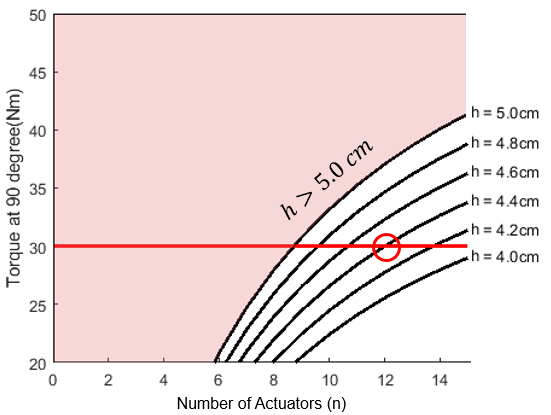
\includegraphics[width=0.45\textwidth]{dif_R_n.PNG}
\caption{Various actuator heights and quantities plotted against each other to assess potential solutions to finding the optimum parameters that would yield 30$N \cdot m$ of torque.}
\vspace{-1.5em}
\label{fig:dif_R_n}

\end{figure}

%\begin{table}[h]
%\caption{Design parameters. 
%}
%\label{Functional Requirements}
%\begin{center}
%\renewcommand{\arraystretch}{1.5} % Default value: 1
%\begin{tabular}{| c | c | c | c |}
%\hline
%\textbf{Distance} & \textbf{Height}  & \textbf{Width} & \textbf{Number}\\ 

%\hline%

%8mm &  44mm  & 75mm & 12 Actuators\\ 

%\hline

%\end{tabular}
%\end{center}
%\end{table}


\section{EXPERIMENTAL METHODS AND RESULTS}

\subsection{Actuator Stiffness}

A single actuator is placed in a uniaxial tensile strength machine ( model make location) and fixed between compression platens to investigate strength and stiffness.  The platens are offset 8mm apart, allowing the actuator the same spacing as when it is in the actuator array.  A series of five experiments was performed on the actuator by inflating it up to a pressure of 300kPa in 20kPa increments. A linear relation between the force output and the internal pressure of the actuator and an average maximum force of 567.8N +/- 3.56N was observed. The stiffness of the actuator was then tested, inflated to the maximum tested pressure of 300kPa,  and then placed between the two platens  This produced an average force output of 550 N over the area of the platen ($1509.43mm^2$) (Fig. 11).  

Secondly, using the same force measured in the first test as a threshold, the actuator was compressed in the same axis and displaced 19.5 mm, providing a maximum stiffness of 28.2 kN/m calculated from the relationship of the force applied and the displacement achieved. The stiffness test demonstrated the extremely high force to weight ratio of this particular actuator design, with a single actuator weighing only 7.1g, including the weight of the metal push-to-connect fitting. 


\begin{figure}[t!]
\centering
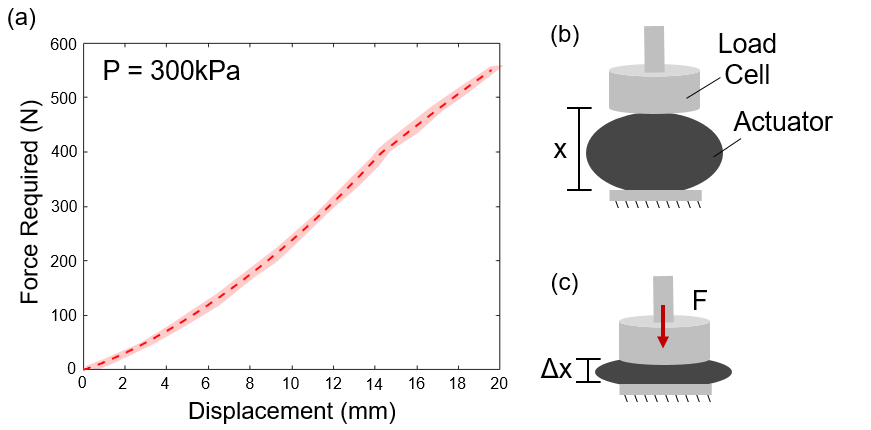
\includegraphics[width=0.5\textwidth]{stiiffnesstest.PNG}
\caption{Testing of individual air bladder, with the total pushing force of a single actuator constrained at 8mm - the distance each bladder sits apart from adjacent bladders in the array of bladders in the flexion actuator.}
\label{fig:stifftest}
\end{figure}

\subsection{Torque verification and comparison
}

\begin{figure} [b!]
\centering
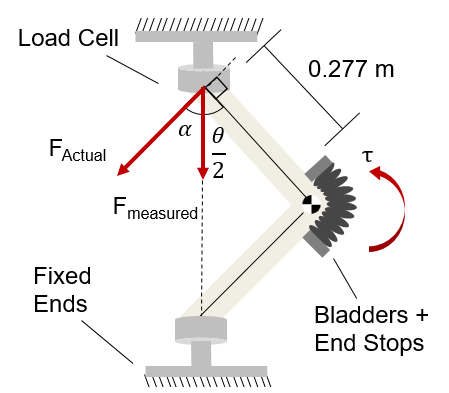
\includegraphics[width=0.3\textwidth]{torquetest.PNG}
\caption{Test setup for the torque measurements of the array of actuators
}
\label{fig:t_test}
\end{figure}

\begin{figure}
\centering
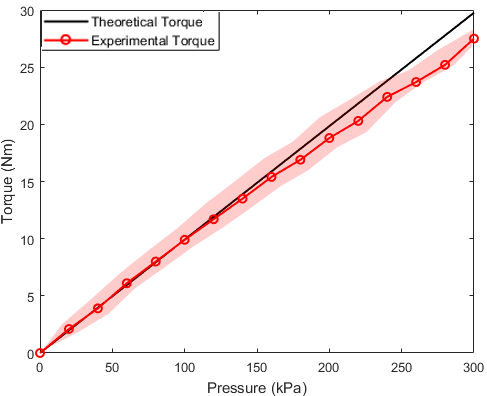
\includegraphics[width=0.4\textwidth]{Torque_stuff3.PNG}
\caption{Torque output of the exosuit in the actuator array shows a comparison of the two linear systems with an average error of 6\% until roughly 200kPa, where the error increases to 11\%}
\label{fig:torques}
\vspace{-1.5em}
\end{figure}

To verify the torque output compared to the theoretical model, the exosuit is mounted on an analog joint and placed in a universal testing machine with the joint angle fixed at 90 degrees \ref{fig:t_test}. The actuator array is inflated in increments of 25kPa up to the maximum of 275kPa, at which point the device is predicted to reach its final torque output of 30 $N\cdot m$.  The device is loaded and unloaded to test for the presence of hysteresis, which was minor and overall negligible as it followed a similar line as the loading of the exosuit.  The forces measured represent the maximum transmittance of forces to the human body when it is assumed the user will be lifting a safe, maximum weight with a single arm. The system was able to reach a maximum of 27.6 $\pm$ 0.67 $N\cdot m$ of torque, which is less than a 10\% error for the predicted 30$N \cdot m$ of torque. A linear regression model was used to compare the results to the theoretical model, and showed an average error of 6\% until 200kPa, at which the margin of error increased to about 11\%, likely due to the array lifting or the actuators slipping from their original orientation with higher interaction forces (Fig. \ref{fig:torques}).  

%No R2, talk about % error between theoretical and measured
\section{PARTICIPANT TESTING}

Participant testing was conducted in order to verify the design conditions of the exosuit and effectiveness of the device. Surface electromyography (sEMG) (model make location) measurement and Motion capture (model make location) were utilized for recording muscle activity and bending angles, respectively. A single female participant, age: 23 years, height: 1.67 m, weight: 52 kg, lifted predetermined weights with and without assistance. All tests were conducted with a resting interval of two minutes between series of tests with the participant’s forearm supinated. 

\begin{figure}[b!]
\centering
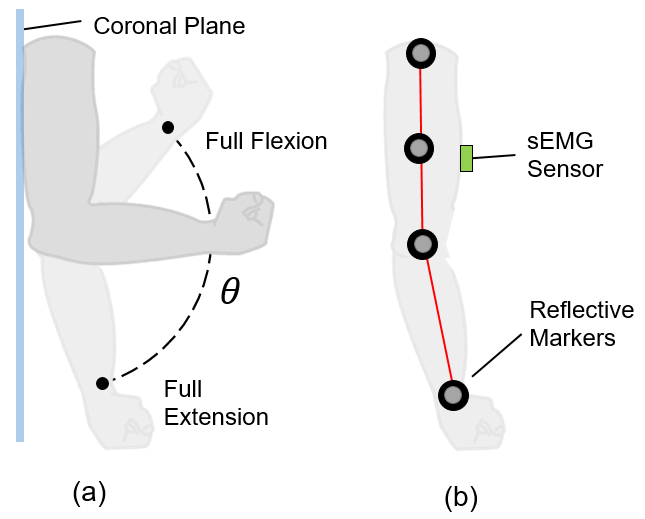
\includegraphics[width=0.3\textwidth]{sEMG.PNG}
\caption{Geometric analytical model of actuator behavior patterns in varying configurations of sizes}
\label{fig:sEMG}
\end{figure}

\begin{figure*}[t]
\centering
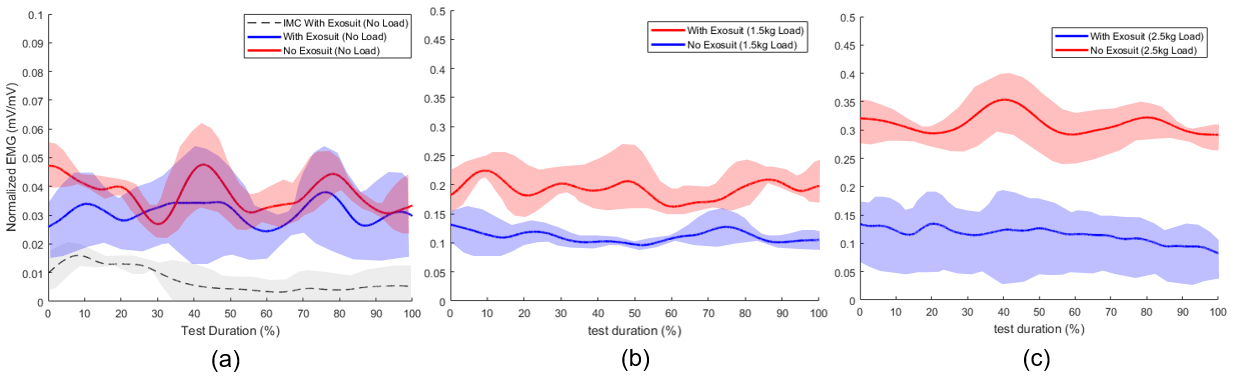
\includegraphics[width=\textwidth]{EMG_Stuff.PNG}
\caption{(a) and (b) Normalized EMG readings of muscle strain during lifting of 2.5kg and 1.5kg, respectively, with and without the assistance from the exosuit. Reduction in measured muscle activity is not seen to be proportional to the load.  (c) Any discrepancy is likely the result of needing to support the mass of the device.}
\label{fig:EMG}
\vspace{-1.5em}
\end{figure*}
EMG data was normalized to readings from maximum voluntary contraction (MVC) and a fully relaxed arm. Measured MVC correlated to an average of 73.6N of force generated by the bicep at a 90$^o$ elbow angle with the upper arm lying on the coronal plane. Reflective markers were fixed at the: top of the shoulder (acromion), center of upper arm (humerus), elbow’s axis of rotation (medial epicondyle), and wrist (styloid process) (Fig. \ref{fig:sEMG}). Bending angle of the elbow was measured relative to the axis of upper arm’s markers. 

The current control method of exosuit actuation was built on an single-input-single-output (SISO) open loop system. Pressure was manually defined by an adjustable analog regulator and monitored.


\subsection{Assisted Lift Test}

This test to verifies lifting assistance the elbow exosuit was capable of producing when worn on a healthy participant. The procedure includes two sets of tests for measuring muscle activity while supporting a mass of 1.5kg and 2.5kg, both assisted and unassisted by the exosuit. Additionally, baseline readings with no load, with and without the device, as well as actuation to support the weight of the user’s forearm were measured. All tests were conducted with the subjects upper arm resting against a vertical surface to ensure there was no deflection from the coronal plane and is also used as the line of reference for measuring the arm’s bending angle. 

The participant gripped the known weights with the arm relaxed. Pressure was increased until a 90$^o$ bend was obtained, determined by a marker fixed in front of the subject. This position was held for five seconds where the data within this time-frame was analyzed for steady-state muscle activity post-motion.  

Results of the test indicate the exosuit is not only capable of supporting loads borne by the user, but also shows that the device is unrestricting when actuated to 90$^o$ as shown in Fig. \ref{fig:EMG}. Both load bearing results are in agreement with maximum MVC EMG readings, with the 1.5kg and 2.5kg weights showing 19.2\% and 31.2\% muscle activity, respectively. Muscle activity reduction from exosuit assistance, however did not see complete nullification of muscle strain where a reduction of 8.2\% and 19.7\% strain was measured for the support of 1.5kg and 2.5kg masses. It should be noted, that the averaged EMG signal from device assistance was approximately equal at 11.5\% and 11.3\%. This is indicative of the bicep brachii contracting due to the participant stiffening the wrist in order to maintain hand-forearm parallelism while supporting the weight[FIND CITATION]. This behavior was not correlated to the exosuit due to the compliance of the materials, since further tests showed only 0.5\% muscle activity from the exosuit lifting and supporting the participant’s arm. 



\subsection{Range of Motion Study}

\begin{figure}[b!]
\centering
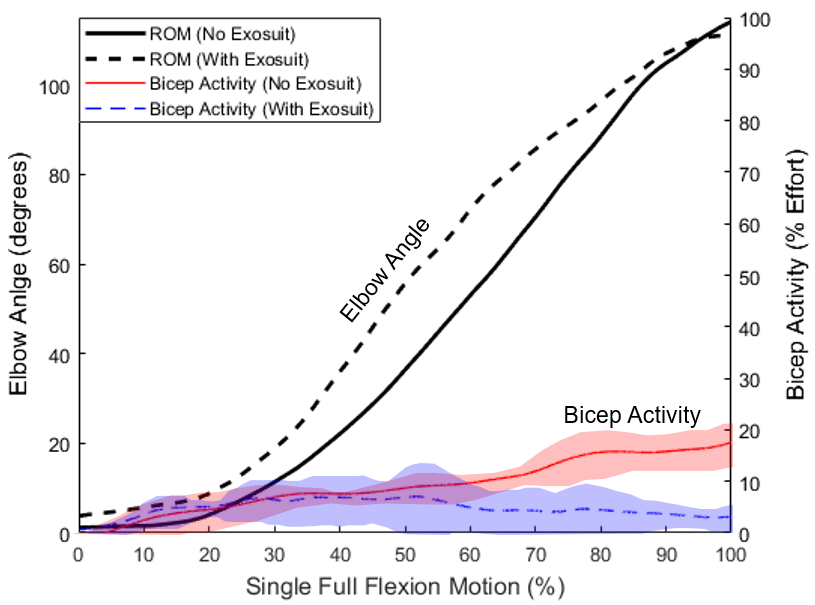
\includegraphics[width=0.4\textwidth]{ROM.PNG}
\caption{Range of Motion of the user while wearing the device and without the device.  The height of the peak is due to the result of the dynamic test, and is representative of the participant lifting and accelerating the weight of their own, unloaded arm against gravity.
}
\vspace{-1.5em}
\label{fig:ROM}
\end{figure}

A ROM test is performed to quantify the angles the user’s arm was able to achieve before and after wearing the exosuit to determine how much the exosuit impede the user’s ROM.   Additionally, an EMG sensor was used to measure the muscle activity through the entire range of motion test both with the exosuit and without to verify that the user was receiving assistance from the exosuit until the full flexion motion had been achieved.  A motion capture system was used to track the user’s movement through the motion of a single ‘curl’ from full elbow extension to full elbow flexion while in supination.  The user performed a single curl with no assistance from the exosuit.  The user was then asked to perform the same type of motion relying on device to perform the entire range of motion for them.  The position of the upper arm and elbow markers were treated as the vector $\textbf{V1}$ shown in Fig. 13, while the markers from the elbow to the forearm were treated as the vector $\textbf{V2}$.  

The angle between these vectors was calculated through the total range of motion decreased 10 degrees while wearing the device, however the muscle activity decreased by 90.9\% of the original effort exerted to achieve almost the same range of motion (Fig. \ref{fig:ROM}.  While the total range of motion may have been impacted slightly, the reduction in muscle activity decreased significantly to show the device was able to provide active assist through the majority of the full range of motion with negligible assistance from the participants bicep.   

\section{CONCLUSIONS}

In this paper, the design, characterization, and evaluation of a lightweight soft robotic elbow exosuit was presented, aimed to assist in elbow flexion of warehouse workers. The design of the device was composed of an array of overlapping actuators enclosed in an inelastic fabric casing to assist the flexion motion. These actuators were tested and characterized for their force output on the experimental test setup.  From the results of the tests detail in section X, it was observed that the device was able to perform the primary task of providing nearly 28$N \cdot m$ of torque about an elbow joint, within 10\% error of the predicted 30$N \cdot m$, with the dimensions chosen based off of the parameters chosen from the modeling of the system.  The design of the actuators allowed for extremely high force-to-weight ratios, providing a maximum stiffness of 28.2kN/m per actuator when inflated to 300kPa.  

	Limitation of the device were related to how higher forces were translated to the body.  While the exosuit was able to produce 27.6Nm of torque about the elbow joint, there were ergonomics complications when actually worn on the human body that could not be represented in the models.  Because of the compliance of the human tissue and muscle, the device became restrictive, even when showing it was able to provide a reduction in muscles activity for more realistic loads for the user.  

The next steps for the exosuit are to implementation of user intent and send signals to the corresponding actuators based on the needed motion for the users based on EMG signals.  Additional steps would investigate a mobile actuation system, which could be worn by the user or actuate the exosuit through existing pneumatic systems.  
% mention using simulations fin a future design iteration

\addtolength{\textheight}{-12cm}   % This command serves to balance the column lengths
                                  % on the last page of the document manually. It shortens
                                  % the textheight of the last page by a suitable amount.
                                  % This command does not take effect until the next page
                                  % so it should come on the page before the last. Make
                                  % sure that you do not shorten the textheight too much.

%%%%%%%%%%%%%%%%%%%%%%%%%%%%%%%%%%%%%%%%%%%%%%%%%%%%%%%%%%%%%%%%%%%%%%%%%%%%%%%%



%%%%%%%%%%%%%%%%%%%%%%%%%%%%%%%%%%%%%%%%%%%%%%%%%%%%%%%%%%%%%%%%%%%%%%%%%%%%%%%%



%%%%%%%%%%%%%%%%%%%%%%%%%%%%%%%%%%%%%%%%%%%%%%%%%%%%%%%%%%%%%%%%%%%%%%%%%%%%%%%%
%%%%%%%%%%%%%%%%%%%%%%%%%%%%%%%%%%%%%%%%%%%%%%%%%%%%%%%%%%%%%%%%%%%%%%%%%%%%%%%%


% ********************************** Bibliography ******************************

\bibliographystyle{plain}
%\bibliographystyle{plainnat} % use this to have URLs listed in References
% \cleardoublepage
\bibliography{Lib} % Path to your References.bib file



% \begin{thebibliography}{99}

% \bibitem{c1} G. O. Young, ÒSynthetic structure of industrial plastics (Book style with paper title and editor),Ó 	in Plastics, 2nd ed. vol. 3, J. Peters, Ed.  New York: McGraw-Hill, 1964, pp. 15Ð64.
% \bibitem{c2} W.-K. Chen, Linear Networks and Systems (Book style).	Belmont, CA: Wadsworth, 1993, pp. 123Ð135.
% \bibitem{c3} H. Poor, An Introduction to Signal Detection and Estimation.   New York: Springer-Verlag, 1985, ch. 4.
% \bibitem{c4} B. Smith, ÒAn approach to graphs of linear forms (Unpublished work style),Ó unpublished.
% \bibitem{c5} E. H. Miller, ÒA note on reflector arrays (Periodical styleÑAccepted for publication),Ó IEEE Trans. Antennas Propagat., to be publised.
% \bibitem{c6} J. Wang, ÒFundamentals of erbium-doped fiber amplifiers arrays (Periodical styleÑSubmitted for publication),Ó IEEE J. Quantum Electron., submitted for publication.
% \bibitem{c7} C. J. Kaufman, Rocky Mountain Research Lab., Boulder, CO, private communication, May 1995.
% \bibitem{c8} Y. Yorozu, M. Hirano, K. Oka, and Y. Tagawa, ÒElectron spectroscopy studies on magneto-optical media and plastic substrate interfaces(Translation Journals style),Ó IEEE Transl. J. Magn.Jpn., vol. 2, Aug. 1987, pp. 740Ð741 [Dig. 9th Annu. Conf. Magnetics Japan, 1982, p. 301].
% \bibitem{c9} M. Young, The Techincal Writers Handbook.  Mill Valley, CA: University Science, 1989.
% \bibitem{c10} J. U. Duncombe, ÒInfrared navigationÑPart I: An assessment of feasibility (Periodical style),Ó IEEE Trans. Electron Devices, vol. ED-11, pp. 34Ð39, Jan. 1959.
% \bibitem{c11} S. Chen, B. Mulgrew, and P. M. Grant, ÒA clustering technique for digital communications channel equalization using radial basis function networks,Ó IEEE Trans. Neural Networks, vol. 4, pp. 570Ð578, July 1993.
% \bibitem{c12} R. W. Lucky, ÒAutomatic equalization for digital communication,Ó Bell Syst. Tech. J., vol. 44, no. 4, pp. 547Ð588, Apr. 1965.
% \bibitem{c13} S. P. Bingulac, ÒOn the compatibility of adaptive controllers (Published Conference Proceedings style),Ó in Proc. 4th Annu. Allerton Conf. Circuits and Systems Theory, New York, 1994, pp. 8Ð16.
% \bibitem{c14} G. R. Faulhaber, ÒDesign of service systems with priority reservation,Ó in Conf. Rec. 1995 IEEE Int. Conf. Communications, pp. 3Ð8.
% \bibitem{c15} W. D. Doyle, ÒMagnetization reversal in films with biaxial anisotropy,Ó in 1987 Proc. INTERMAG Conf., pp. 2.2-1Ð2.2-6.
% \bibitem{c16} G. W. Juette and L. E. Zeffanella, ÒRadio noise currents n short sections on bundle conductors (Presented Conference Paper style),Ó presented at the IEEE Summer power Meeting, Dallas, TX, June 22Ð27, 1990, Paper 90 SM 690-0 PWRS.
% \bibitem{c17} J. G. Kreifeldt, ÒAn analysis of surface-detected EMG as an amplitude-modulated noise,Ó presented at the 1989 Int. Conf. Medicine and Biological Engineering, Chicago, IL.
% \bibitem{c18} J. Williams, ÒNarrow-band analyzer (Thesis or Dissertation style),Ó Ph.D. dissertation, Dept. Elect. Eng., Harvard Univ., Cambridge, MA, 1993. 
% \bibitem{c19} N. Kawasaki, ÒParametric study of thermal and chemical nonequilibrium nozzle flow,Ó M.S. thesis, Dept. Electron. Eng., Osaka Univ., Osaka, Japan, 1993.
% \bibitem{c20} J. P. Wilkinson, ÒNonlinear resonant circuit devices (Patent style),Ó U.S. Patent 3 624 12, July 16, 1990. 


% \end{thebibliography}




\end{document}
